%%%%%%%%%%%%%%%%%%%%%%%%%%%%%%%%%%%%%%%%%%%%%%%%%%%%%%%%%%%%%%%%%%%%%%%%%%%%%%%%%%%%%%%%%%%%%%%%%%%%%%%%%%%%%%%%%%%%%%%%%%%%%%%%%%%%%%%%%%%%%%%%%%%%%%%%%%%%%%%%%%%%%%%%%%%%%%%%%%%%%%%%%%%%%%%%%%%%%%%%%%%%%%%%%%%%%%%%%%%%%%%%%%%
%%%%%%%%%%%%%%%%%%%%%%%%%%%%%%%%%%%%%%%%%%%%%%%%%%%%%%%%%%%%%%%%%%%%%%%%%%%%%%%%%%%%%%%%%%%%%%%%%%%%%%%%%%%%%%%%%%%%%%%%%%%%%%%%%%%%%%%%%%%%%%%%%%%%%%%%%%%%%%%%%%%%%%%%%%%%%%%%%%%%%%%%%%%%%%%%%%%%%%%%%%%%%%%%%%%%%%%%%%%%%%%%%%%
%%%%%%%%%%%%%%%%%%%%%%%%%%%%%%%%%%%%%%%%%%%%%%%%%%%%%%%%%%%%%%%%%%%%%%%%%%%%%%%%%%%%%%%%%%%%%%%%%%%%%%%%%%%%%%%%%%%%%%%%%%%%%%%%%%%%%%%%%%%%%%%%%%%%%%%%%%%%%%%%%%%%%%%%%%%%%%%%%%%%%%%%%%%%%%%%%%%%%%%%%%%%%%%%%%%%%%%%%%%%%%%%%%%
\chapter{The Large Hadron Collider}

The Large Hadron Collider (LHC)~\cite{bib:LHC_machine_2008,bib:LHC_2004} is a particle accelerator installed in the former LEP~\cite{bib:LEP_design_1984} tunnel at CERN~\cite{bib:CERN:web}.
It is 26.7~\km in circumference and consists out of two separate rings, which are, in periods of operation, inhabited by two counter-circulating beams.
At the interaction points of the two beams, either proton-proton collisions or heavy ion collisions take place.
In this thesis, only collision data from the year 2012 is analysed.
Thus all machine values cited in the following chapters and paragraphs refer to the setup in 2012 (if not stated otherwise).

The beams are separated into bunches which rotate with a bunch spacing of 50\ns corresponding to a collision frequency of 20\mhz.
Before the bunches are actually filled into the LHC rings they are pre-accelerated in other accelerators, which are (in the order they are actually passed by the protons) Linac2, Proton  Synchrotron Booster (PSB), Proton Synchrotron (PS), Super Proton Synchrotron (SPS).
The injector chain and the LHC ring with its experiments is visualised in Fig~\ref{fig:LHC}.
\begin{figure}[!b]
  \centering
      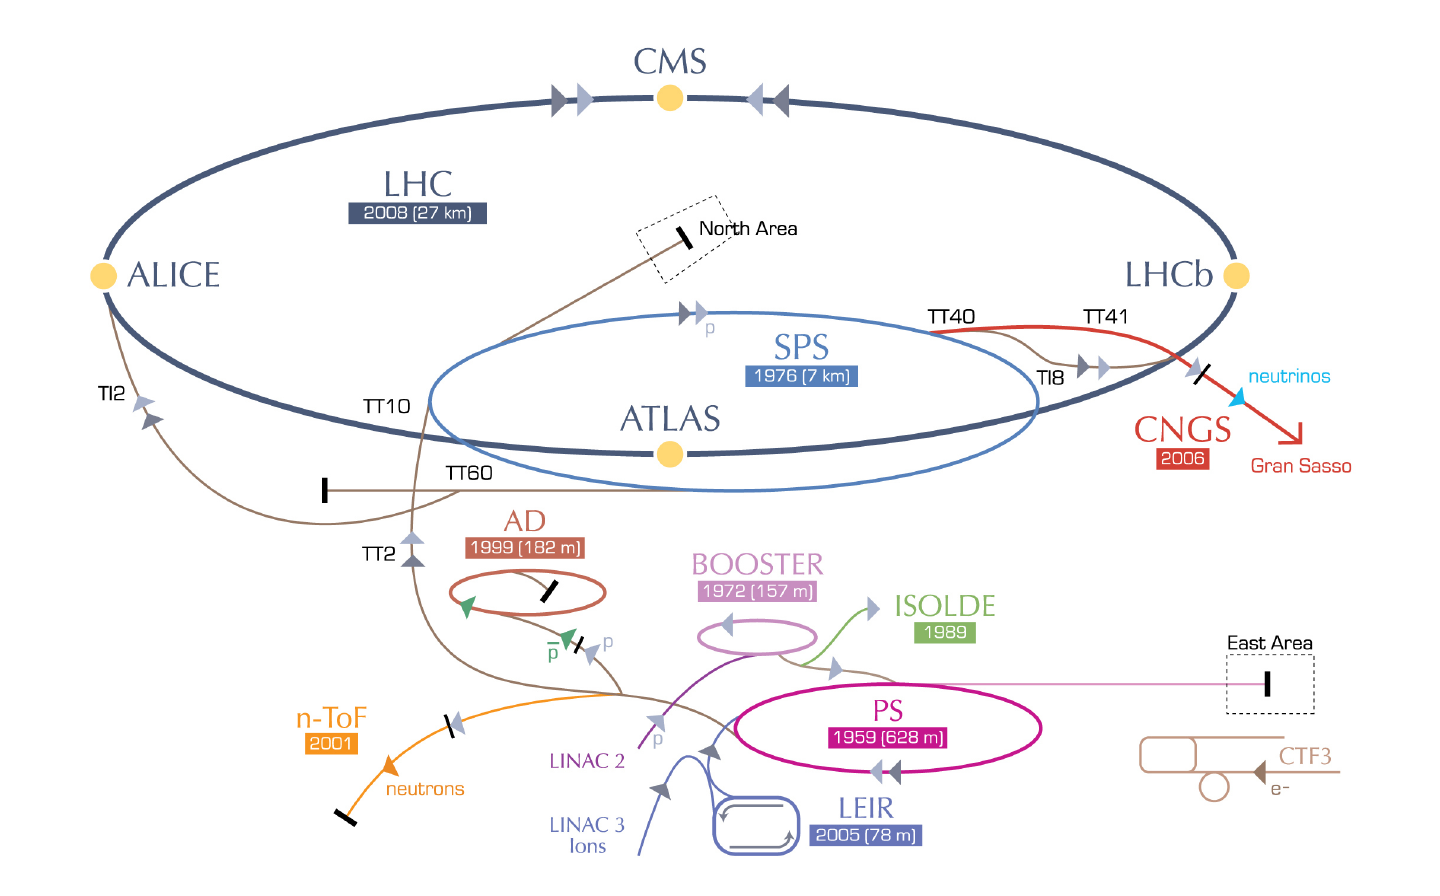
\includegraphics[width=0.79\textwidth]{figures/experiment/LHC/LHC_small.png}
  \caption{Visualisation of the LHC with its experiments and the injector chain. Taken from~\cite{bib:CERNBrochure}.}  
  \label{fig:LHC}
\end{figure}

In the LHC, the beams are kept on the circuit with the help of a magnetic field of 4.76\tesla.
Further quadrupole and sextupole magnets squeeze and focus the bunches.
They have a spread of roughly 8\cm length and a Gaussian shape radius of 20\mum RMS at the interaction point.
The number of contained protons in each bunch is of the order $10^{11}$.
The LHC has eight different insertion region, where four of them are dedicated to the four main experiments of the LHC, the CMS, ATLAS, LHCb and ALICE experiments.
The CMS~\cite{bib:CMS:experiment,bib:CMS:TDR} and ATLAS~\cite{bib:ATLAS:experiment,bib:ATLAS:TDR_1,bib:ATLAS:TDR_2} experiments are so-called ``general purpose experiments'', not designed for one specific task.
In contrary, the LHCb~\cite{bib:LHCb:experiment} and the ALICE~\cite{bib:ALICE:experiment} experiment are designed with an emphasis on CP-violation measurements and heavy ion collisions, respectively.
Each experiment is interested thus in different processes to happen at the beam collision points.
The number of expected event for a given process can be expressed in terms of the corresponding cross section $\sigma$ times the integrated luminosity.
\begin{equation}
N = L \cdot \sigma,
\end{equation}
with an integrated luminosity of $L=\int \mathcal{L}\, dt$, where $\mathcal{L}$ is the instantaneous luminosity (which can change over time).

The instantaneous luminosity $\mathcal{L}$ depends on the several machine parameters, such as the collision frequency $f$, the number of particles in the bunches $n_1$ and $n_2$,
the spread in the transverse plane of the bunches $\sigma_x$ and $\sigma_y$ and a geometrical correction parameter $F$ due to the crossing angle of the two bunches at the interaction point
\begin{equation}
\mathcal{L} = \frac{f n_1 n_2 }{4 \pi \sigma_x \sigma_y} \cdot F.
\end{equation}
In 2012, the peak luminosity was $7.7 \cdot 10^{33} \frac{1}{\text{cm}^2\,\text{s}}$.
The total integrated luminosity over time recorded at the CMS experiment is shown in Fig.~\ref{fig:Lumi}.

\begin{figure}[!b]
  \centering
      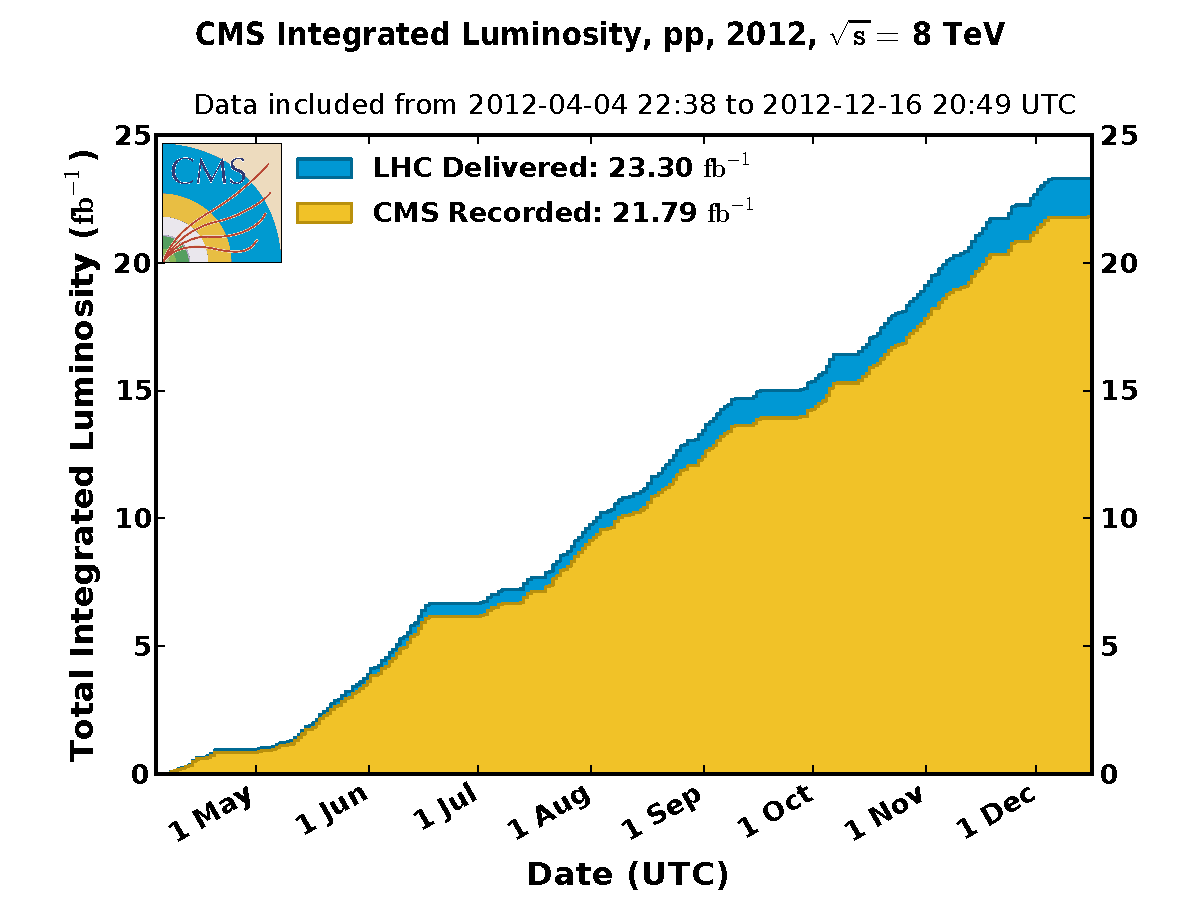
\includegraphics[width=0.59\textwidth]{figures/experiment/LHC/int_lumi_per_day_cumulative_pp_2012.pdf}
  \caption{Integrated luminosity delivered by LHC (blue) and recorded by CMS (orange) in the year 2012. Taken from~\cite{bib:LumiWiki}.}  
  \label{fig:Lumi}
\end{figure}






%%%%%%%%%%%%%%%%%%%%%%%%%%%%%%%%%%%%%%%%%%%%%%%%%%%%%%%%%%%%%%%%%%%%%%%%%%%%%%%%%%%%%%%%%%%%%%%%%%%%%%%%%%%%%%%%%%%%%%%%%%%%%%%%%%%%%%%%%%%%%%%%%%%%%%%%%%%%%%%%%%%%%%%%%%%%%%%%%%%%%%%%%%%%%%%%%%%%%%%%%%%%%%%%%%%%%%%%%%%%%%%%%%%
%%%%%%%%%%%%%%%%%%%%%%%%%%%%%%%%%%%%%%%%%%%%%%%%%%%%%%%%%%%%%%%%%%%%%%%%%%%%%%%%%%%%%%%%%%%%%%%%%%%%%%%%%%%%%%%%%%%%%%%%%%%%%%%%%%%%%%%%%%%%%%%%%%%%%%%%%%%%%%%%%%%%%%%%%%%%%%%%%%%%%%%%%%%%%%%%%%%%%%%%%%%%%%%%%%%%%%%%%%%%%%%%%%%
%%%%%%%%%%%%%%%%%%%%%%%%%%%%%%%%%%%%%%%%%%%%%%%%%%%%%%%%%%%%%%%%%%%%%%%%%%%%%%%%%%%%%%%%%%%%%%%%%%%%%%%%%%%%%%%%%%%%%%%%%%%%%%%%%%%%%%%%%%%%%%%%%%%%%%%%%%%%%%%%%%%%%%%%%%%%%%%%%%%%%%%%%%%%%%%%%%%%%%%%%%%%%%%%%%%%%%%%%%%%%%%%%%%
\FloatBarrier
\chapter{CMS detector}
The Compact Muon Solenoid (CMS) detector~\cite{bib:CMS:experiment,bib:CMS:TDR} is a general purpose detector, designed to explore particle physics phenomena up to the multi-TeV scale.
The detector concept is an onion-like structure of different layers, each one made up with a different type of detector.
In Fig.~\ref{fig:CMSdetector}, a perspective view of the CMS detector is depicted. 
\begin{figure}[!b]
  \centering
      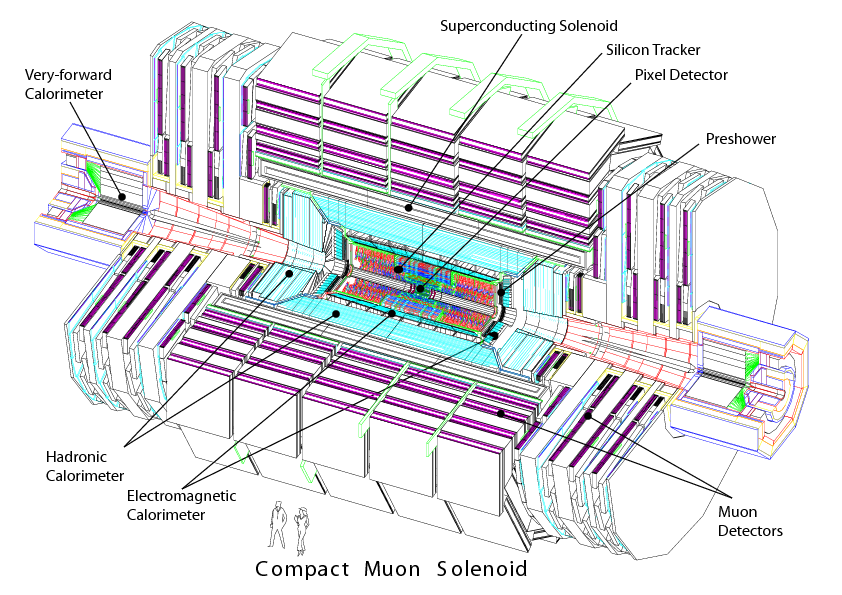
\includegraphics[width=0.99\textwidth]{figures/experiment/CMS/cms_complete_labelled.png}
  \caption{A perspective view of the CMS detector. Taken from~\cite{bib:CMS:experiment}}  
  \label{fig:CMSdetector}
\end{figure}
The used coordinate system at the CMS experiment consists of the pseudorapidity $\eta = -\ln \tan{\frac{\theta}{2}}$ and the azimuthal angle $\phi$.
The advantage of the pseudorapidity $\eta$ is the Lorentz invariance with respect to the z-axis (beam axis).
The angle $\phi$ covers the direction in the $x-y$ plane (orthogonal to the beam axis).

In the following, the various detector components of the CMS detector from the inside to the outside will be explained.

\FloatBarrier
\section{The tracking system}
The tracking system is really important!
\subsection*{The silicon pixel tracker}
\subsection*{The silicon strip tracker}

\section{The calorimeters}
\subsection*{The electromagnet calorimeter}
\subsection*{The Hadronic calorimeter}

\section{The muon system}

\section{The trigger system}

\begin{itemize}
\item General purpose detector (picture) - short overview (tarcker, calorimeters, etc), pseudorapittyt and phi and z
\item Tracker (Pixel tracker - silicon strip tracker - energy measurements in the tracker )
\item Calorimeter - eCAL and HCAL
\item Muon system
\item Trigger system
\item 10 pages
\end{itemize}

%%%%%%%%%%%%%%%%%%%%%%%%%%%%%%%%%%%%%%%%%%%%%%%%%%%%%%%%%%%%%%%%%%%%%%%%%%%%%%%%%%%%%%%%%%%%%%%%%%%%%%%%%%%%%%%%%%%%%%%%%%%%%%%%%%%%%%%%%%%%%%%%%%%%%%%%%%%%%%%%%%%%%%%%%%%%%%%%%%%%%%%%%%%%%%%%%%%%%%%%%%%%%%%%%%%%%%%%%%%%%%%%%%%
%%%%%%%%%%%%%%%%%%%%%%%%%%%%%%%%%%%%%%%%%%%%%%%%%%%%%%%%%%%%%%%%%%%%%%%%%%%%%%%%%%%%%%%%%%%%%%%%%%%%%%%%%%%%%%%%%%%%%%%%%%%%%%%%%%%%%%%%%%%%%%%%%%%%%%%%%%%%%%%%%%%%%%%%%%%%%%%%%%%%%%%%%%%%%%%%%%%%%%%%%%%%%%%%%%%%%%%%%%%%%%%%%%%
%%%%%%%%%%%%%%%%%%%%%%%%%%%%%%%%%%%%%%%%%%%%%%%%%%%%%%%%%%%%%%%%%%%%%%%%%%%%%%%%%%%%%%%%%%%%%%%%%%%%%%%%%%%%%%%%%%%%%%%%%%%%%%%%%%%%%%%%%%%%%%%%%%%%%%%%%%%%%%%%%%%%%%%%%%%%%%%%%%%%%%%%%%%%%%%%%%%%%%%%%%%%%%%%%%%%%%%%%%%%%%%%%%%
\FloatBarrier
\chapter{Event reconstruction and particle identification}

Event reconstruction relies on very complicated algorthms bla


%%%%%%%%%%%%%%%%%%%%%%%%%%%%%%%%%%%%%%%%%%%%%%%%%%%%%%%%%%%%%%%%%%%%%%%%%%%%%%%%%%%%%%%%%%%%%%%%%%%%%%%%%%%%%%%%%%%%%%%%%%%%%%%%%%%%%%%%%%%%%%%%%%%%%%%%%%%%%%%%%%%%%%%%%%%%%%%%%%%%%%%%%%%%%%%%%%%%%%%%%%%%%%%%%%%%%%%%%%%%%%%%%%%
%%%%%%%%%%%%%%%%%%%%%%%%%%%%%%%%%%%%%%%%%%%%%%%%%%%%%%%%%%%%%%%%%%%%%%%%%%%%%%%%%%%%%%%%%%%%%%%%%%%%%%%%%%%%%%%%%%%%%%%%%%%%%%%%%%%%%%%%%%%%%%%%%%%%%%%%%%%%%%%%%%%%%%%%%%%%%%%%%%%%%%%%%%%%%%%%%%%%%%%%%%%%%%%%%%%%%%%%%%%%%%%%%%%
%%%%%%%%%%%%%%%%%%%%%%%%%%%%%%%%%%%%%%%%%%%%%%%%%%%%%%%%%%%%%%%%%%%%%%%%%%%%%%%%%%%%%%%%%%%%%%%%%%%%%%%%%%%%%%%%%%%%%%%%%%%%%%%%%%%%%%%%%%%%%%%%%%%%%%%%%%%%%%%%%%%%%%%%%%%%%%%%%%%%%%%%%%%%%%%%%%%%%%%%%%%%%%%%%%%%%%%%%%%%%%%%%%%
\FloatBarrier
\chapter{Event simulation}
